% !TeX root = ../libro.tex
% !TeX encoding = utf8

\setchapterpreamble[c][0.75\linewidth]{%
	\sffamily
  Definiremos los conceptos más relevantes para el estudio del conjunto de datos al que se han aplicado los modelos.
	\par\bigskip
}
\chapter{Conjunto de datos}\label{Conjunto}

\section{Conceptos genéticos relevantes}\label{st:conceptos-geneticos}
Las cuatro bases nitrogenadas, también llamadas \textbf{nucleótidos}, que se encuentran en el ADN son Adeninda (A), Guanina (G), Citosina (C) y Timina (T) y son las unidades estructurales básicas del genoma. A la mutación de una sola posición de un nucleótido se la llama \textbf{\textit{Single Nucleotide Polymorphism}} (SNP) y a cada posible tipo nucleótido se le llama \textbf{alelo}. Normalmente los SNPs son bialélicos, es decir, sólo presentan dos posibles tipos de nucleótidos y de éstos, los SNPs se suelen referir sólo a los que tengan una frecuencia de alelo menos común (\textit{MAF} en inglés) mayor al 1\%. Definimos esta frecuencia como la frecuencia del segundo alelo más común en un determinado \textbf{locus} (posición de un SNP o gen en un cromosoma), que para los SNPs bialélicos será el alelo menos común y para los trialélicos o tetralélicos se tomará el segundo más común. Un locus puede ser homocigótico cuando los dos alelos son el mismo y heterocigótico cuando son diferentes. \cite{su2007single}\\
Los SNPs tienen un gran interés en el estudio de enfermedades puesto que representan el 90\% de todas las variaciones genéticas humanas y los SNPs con una MAF de al menos el 1\% ocurre cada 100 o 300 bases del genoma humano que tiene unas 3000 millones de pares de bases. A pesar de que estas variaciones del ADN humano representan menos de un 1\% (el 99\% restante es igual en toda la población), pueden tener un mayor impacto en cómo los humanos responden a enfermedades, haciendo de los SNPs unos valores muy importantes para el desarrollo de medicinas o para el diagnóstico médico. \cite{su2007single}\\
Los SNPs también han demostrado ser relevantes a la hora de encontrar genes relacionados con enfermedades como cáncer, diabetes y el trastorno del espectro autista, que es lo que trabajamos aquí. Sin embargo, es complicado establecer estas relaciones a partir de un sólo gen alterado así que hay que alejarse de los medios convencionales para encontrar estas relaciones, como por ejemplo el \textit{machine learning}. \cite{su2007single}\\\\
Los cromosomas humanos vienen en pares: uno de la madre y otro del padre, y al conjunto de alelos que una persona tiene en un par de cromosomas se le llama \textbf{genotipo} y el \textbf{genotipado} es el método para obtenerlo. El término genotipo puede incluir los alelos del SNP que una persona tiene en un determinado locus o muchos SNPs a lo largo del genoma. Al conjunto de los alelos asociados de los SNPs en el mismo cromosoma se le llama \textbf{haplotipo}.\\
El método más preciso y actual es el \textbf{\textit{Polymerase Chain Reaction}} (PCR), que hace múltiples copias de una secuencia de ADN, hasta la región donde se encuantran los SNPs y luego secuencia la región directamente.\\

Los microarrays son una tecnología para estudiar la expresión de muchos genes a la vez. Han hecho posible identificar, clasificar y asignar funciones a muchos genes no caracterizados, simplemente mediante la determinación de cuándo los genes se expresan o están reprimidos  \cite{microarray}. Son chips de tamaño pequeño con una superficie sólida a la que se le une una colección de fragmentos de ADN. El color y la \textbf{intensidad} de fluorescencia en cada punto permite identificar las diferencias genéticas clave. Esta intensidad es la que se nos da para estudiar en el conjunto de datos.

\begin{figure}[H]
  \centering
  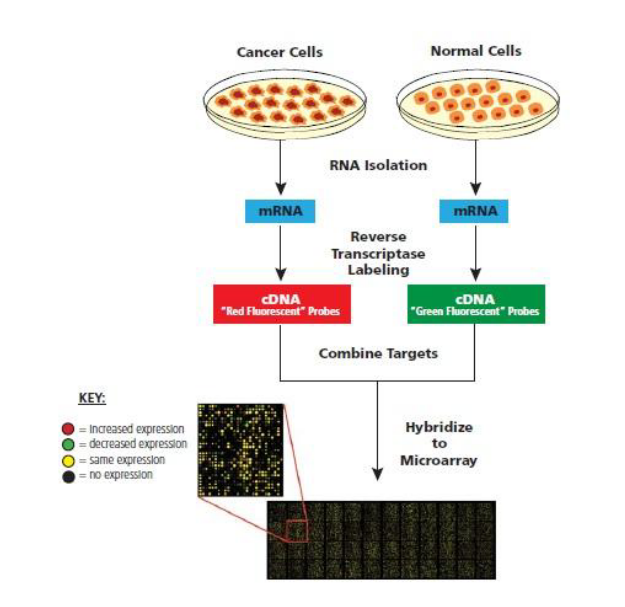
\includegraphics[width=0.8\textwidth]{microarray}
  \caption{Análisis de microarrays. \cite{microarray}}
  \label{fig:overfit}
\end{figure}
\begin{center}
\end{center}

Por último, cabe resaltar el concepto de \textbf{GWAS}. Son siglas en inglés que dan nombre al \textit{estudio de asociación de genoma completo}, un enfoque de la investigación genética para asociar variaciones genéticas con enfermedades. Se trata de analizar el genoma de un gran número de personanas y buscar algún rasgo genético que sirva para predecir la enfermedad. En este caso, el Trastornos del Espectro Autismta (en inglés, \textit{Autism Spectrum Disease}, ASD).

\section{Materiales}\label{st:Materiales}
Definimos ahora en esta sección el conjunto de datos utilizado y en concreto, el conjunto o \textit{dataset} utilizado para el estudio.
\subsection{Conjunto de datos completo}
Los datos de autismo han sido proporcionados por el  National Center for Biotechnology Information (NCBI) a través del \href{https://www.ncbi.nlm.nih.gov/gap/}{\color{blue}{dbGaP}} (por sus siglas, database of Genotypes and Phenotypes) y los datos de control por el \href{https://ega-archive.org/}{\color{blue}{European Genome-Phenome Archive (EGA)}} y vienen distribuidos en archivos con extensión .iou, uno por cada cromosoma (sin contar el sexual) donde cada archivo se compone de una cierta cantidad de filas (individuos, especificados en \autoref{tb:info-datasets}) y 62441 columnas donde las 7 primeras contienen información del individuo y el resto son valores numéricos de las intensidades de los SNPs en ambos alelos. Todos los datos han sido genotipados con el chip de Illumina 1.2 Duo aunque personalizados en algunos SNPs para los datos de ASD lo que hace que no se puedan comparar directamente y es el objeto de estudio de este trabajo.

\begin{table}[H]
  \centering
  \begin{tabular}{ccccc} \toprule
    \multicolumn{5}{c}{Conjunto de datos} \\ \cmidrule(r){1-5}
    Dataset & Otro nombre & Nº Individuos & Plataforma & Nº SNPs          \\ \midrule
    AGP1M & Autism NoDuo & 1194 (398 trios) & ILLUMINA 1M & 1069796          \\ 
    AGP1MDuo & Autism Duo & 2592 (864 trios) & ILLUMINA 1M & 1069796          \\ 
    1958BC & BC & 2930 control individuals & ILLUMINA 1M & 1069796          \\
    NBS & NBS & 2699 control individuals & ILLUMINA 1M & 1069796          \\ \bottomrule
  \end{tabular}
  \caption{Información de los datasets}
  \label{tb:info-datasets}
\end{table}

Los datos y las intensidades han sido extraídas de los ficheros originales en formato IDAT (uno por individuo) con la siguiente descripción de columnas por profesores de la línea de bioinformática del grupo de investigación UTAI:
\begin{itemize}
  \item Columna 1: Código de familia. Es un identificador alfanumérico asignado de forma unívoca a cada trío o familia (hijo y dos padres).
  \item Columna 2: Código del individuo. Identificador único para cada individuo con el formato "n$\_$m" donde n es el código de familia antes mecionado y m el ID.
  \item Columna 3: Código del padre. Representa el ID del padre del individuo. Su valor es $0$ si el individuo no es un hijo.
  \item Columna 4: Código de la madre. El ID de la madre del individuo, que es $0$ si no es un hijo.
  \item Columna 5: Sexo. Vale 1 si el individuo es de sexo masculino y 2 si es femenino.
  \item Columna 6: Estado de afección. Es nuestra variable a predecir, donde $0$ indica paciente sano y 2 enfermo.
  \item Columna 7: Es el mismo código individual de la columna 2.
  \item Columna 8 hasta 7+2*\textit{TotalSNPs}: Valores numéricos de los SNPs. Van por pares representando los pares de alelos.
  \end{itemize}

\subsection{Conjunto de datos estudiado}
Para este trabajo se ha llevado a cabo el estudio del ADN mitocondrial. Los datos, tanto los de trío como los sanos de control vienen dado en archivos .iou, cuyo nombre finaliza en 'Chrom26' ya que se ha trabajado con el cromosoma 26, que hace referencia al material genético mitocondrial. Los datos se presentan con la siguiente estructura:\\
\begin{itemize}
  \item Carpeta 'Autism': Contiene el archivo .iou con el dataset y un archivo .col con los nombres de cada SNP en el mismo orden que aparecen en los pares de columnas.
  \item Carpeta 'NBS': Los primeros datos de control que he usado, también en un archivo.iou. Contiene 2699 individuos sanos con dos posiciones menos de SNPs que los tríos.
  \item Carpeta 'BC': Con 2920 individuos, contiene los segundos datos de control.
  \item Carpeta 'MS': El archivo .col de esta carpeta contiene en orden los nombre de los SNPs para los dos datos de control.
\end{itemize}
Las columnas se describen de la misma forma que en el apartado anterior.\\
Para llevar a cabo el estudio de los datos a través de los modelos predictivos, se deben eliminar las 7 primeras columnas a excepción de la sexta (el estado de afección) como etiqueta a predecir durante el aprendizaje supervisado.\\
Los conjuntos no presentan datos perdidos pero sí hay dos categorías SNPs en el conjunto de los tríos que no están presentes en los datos de control: \textit{mitoc10874t} y \textit{mitog10590a}, que los borramos del conjunto de los tríos para tener exactamente el mismo formato en los tres.\\
En el primer estudio llevado a cabo sólo con los datos de las familias, encontramos que hay 864 afectados (que son los hijos) y 1728 individuos presuntamente sanos (los padres). En el segundo y tercer estudio llevados a cabo con los primeros y segundos datos de control respectivamente, se han eliminado los individuos hijos y se han dejado a los padres marcando su estado de afección con un 2 (afectado) y se han juntado con cada control marcados con 0 (sanos) para predecir qué individuos podrían tener hijos con trastorno del desorden autista (ASD en inglés).
\endinput

%
%
%
%
%
%
%
%
%
%
%
%
%
%
%
%







